\documentclass[../main]{subfiles}
\ifSubfilesClassLoaded{
    \addbibresource{../Biblio/biblio.bib}
    \dominitoc
    \tableofcontentsfile
    \pagenumbering{arabic}
    \setcounter{page}{1}
    \setcounter{chapter}{5}
}{}
\begin{document}
\chapter{Indicateurs numériques de l'apprentissage du modèle d'entrées \label{chap:indicateur}}
\graphicspath{{05-Indicateur/figures},{./figures/}}
\minitoc

\section{Introduction}

Dans les chapitres~\ref{chap:repr} et \ref{chap:analyse}, nous avons identifié des mécanismes caractérisant l'apprentissage d'un modèle d'entrées au sein de l'architecture de cartes en s'appuyant sur les représentations graphiques des poids et des BMU.
Nous avons souligné l'importance de développer des indicateurs numériques pour mesurer cet apprentissage, afin de faciliter la comparaison entre différentes expériences et l'optimisation des paramètres d'apprentissage.

Nous avons représenté les modèles d'entrées à apprendre grâce une variable latente $U$, qui traduit les paramètres libres du modèle d'entrées.
Les représentations graphiques que nous avons étudiées nous ont permis de constater que l'apprentissage du modèle d'entrées dans les architectures de cartes se caractérise par une relation fonctionnelle entre $U$ et la position du BMU $\bmu$ dans chaque carte.
Dans ce chapitre, nous envisageons deux méthodes mesurant la qualité de la relation fonctionnelle entre $U$ et $\bmu$, à savoir le coefficient d'incertitude, qui est une version normalisée de l'information mutuelle, et le ratio de corrélation.
Ces méthodes s'appuient sur la représentation des entrées et réponses des cartes en tant que variables aléatoires.
Nous comparerons leur capacité à traduire la relation fonctionnelle que nous avons observée dans les architectures de deux cartes, afin de déterminer l'indicateur numérique le plus adapté et leurs limitations.

Cependant, nous avons également souligné que pour des architectures de grande taille ou des $U$ de grande dimension, $U$ pourrait ne pas être une fonction de $\bmu$ dans chaque carte. De plus, une représentation distribuée de $U$ entre les cartes, tout en présentant une certaine redondance en terme d'information pourrait être préférable.
Nous discuterons donc en dernière partie de chapitre des possibilités d'utilisation de l'information mutuelle comme indicateur de l'apprentissage du modèle dans une structure de cartes.

\section{\'Eléments de théorie de l'information}

\subsection{Entropie et information mutuelle}

Les notions d'entropie et les valeurs associées, telle que l'information mutuelle entre des variables aléatoires, sont des notions fondamentales de la théorie de l'information de Shannon \parencite{Shannon1948AMT}. Ces quantités sont calculées à partir de la distribution des variables aléatoires.
L'entropie de Shannon d'une variable aléatoire $X$ à valeurs dans un ensemble $\Omega_X$ discret, de distribution $P_X$, est notée $H(X)$ et définie par~: 
\begin{equation}\label{eq:H}
H(X) = - \sum_{x \in \Omega_X}{P_X(x)\textrm{log}(P_X(x))}
\end{equation}

L'entropie de Shannon concerne uniquement des variables discrètes.
Une autre version de l'entropie est définie pour des variables continues, l'entropie différentielle~:
\begin{equation}
    h(X) = - \int_{x \in \Omega_X}{p_X(x)\textrm{log}(p_X(x))dx}
\end{equation}
Avec $p_X$ la densité de probabilité de $X$.
Notons que l'entropie différentielle n'est pas la limite de l'entropie de Shannon calculée par discrétisation de $X$ en $N$ intervalles, $N \rightarrow \infty$. L'entropie différentielle peut prendre des valeurs négatives.

L'existence d'une relation quelconque entre deux variables aléatoires $X,Y$ à valeurs dans $\Omega_X,\Omega_Y$ se mesure par leur \emph{information mutuelle}.
Elle est définie par : 
\begin{equation}\label{eq:MI}
 I(X,Y) = \sum_{x,y \in \Omega_X,\Omega_Y}{P_{XY}(x,y)\textrm{log}(\frac{P_{XY}(x,y)}{P_X(x)P_Y(y)})}
\end{equation}

Avec $P_{XY}$ la distribution de la variable aléatoire jointe $(X,Y)$
Cette valeur mesure la quantité d'information moyenne partagée entre les distributions $X$ et $Y$~: en moyenne, quelle information sur la valeur de $Y$ donne une valeur de $X$ et inversement, quelle information sur la valeur de $X$ donne une valeur de $Y$.

L'information mutuelle possède notamment les propriétés suivantes~:
\begin{enumerate}
\item $I(X,Y) = 0 \Leftrightarrow \textrm{X et Y sont indépendantes}$. L'information mutuelle peut être vue comme une mesure de la distance entre la distribution jointe de $(X,Y)$, $P_{XY}(X,Y)$ et la distribution correspondant à l'indépendance des variables, $P_X(X)P_Y(Y)$.
\item\label{it:h} Elle s'exprime à partir de l'entropie de Shannon : $I(X,Y) = H(X) + H(Y) - H(X,Y) = H(X) - H(X|Y) = H(Y) - H(Y|X)$
\item Elle est symétrique : $I(X,Y) = I(Y,X)$
\item\label{it:eq} Pour toute fonction $f$, $I(X,Y) \geq I(X,f(Y))$. L'égalité est atteinte si et seulement si $f$ est bijective.
\end{enumerate}

L'information mutuelle se calcule également à partir des densités de probabilité pour des variables à valeur continues de densités de probabilité $p_X$ et $p_Y$~:
\begin{equation}
    I(X,Y) = \int_{x \in \Omega_X}\int_{y \in \Omega_Y }{p_{XY}(x,y)\textrm{log}(\frac{p_{XY}(x,y)}{p_X(x)p_Y(y)})dx \: dy}
\end{equation}

Contrairement à l'entropie, la valeur de l'information mutuelle pour des variables continues correspond bien à une limite des valeurs de l'information mutuelle discrète lorsque le nombre de catégories tend vers l'infini \parencite{Cover2005ElementsOI}.
Cependant, dans le cas continu, les propriétés \ref{it:h} et \ref{it:eq} ne sont pas vérifiées. L'information mutuelle n'est en effet pas directement liée à l'entropie différentielle $h$.

\subsection{Méthodes d'estimation}\label{sec:estimation}
\begin{figure}
    \begin{minipage}{0.4\textwidth}
    \centering
    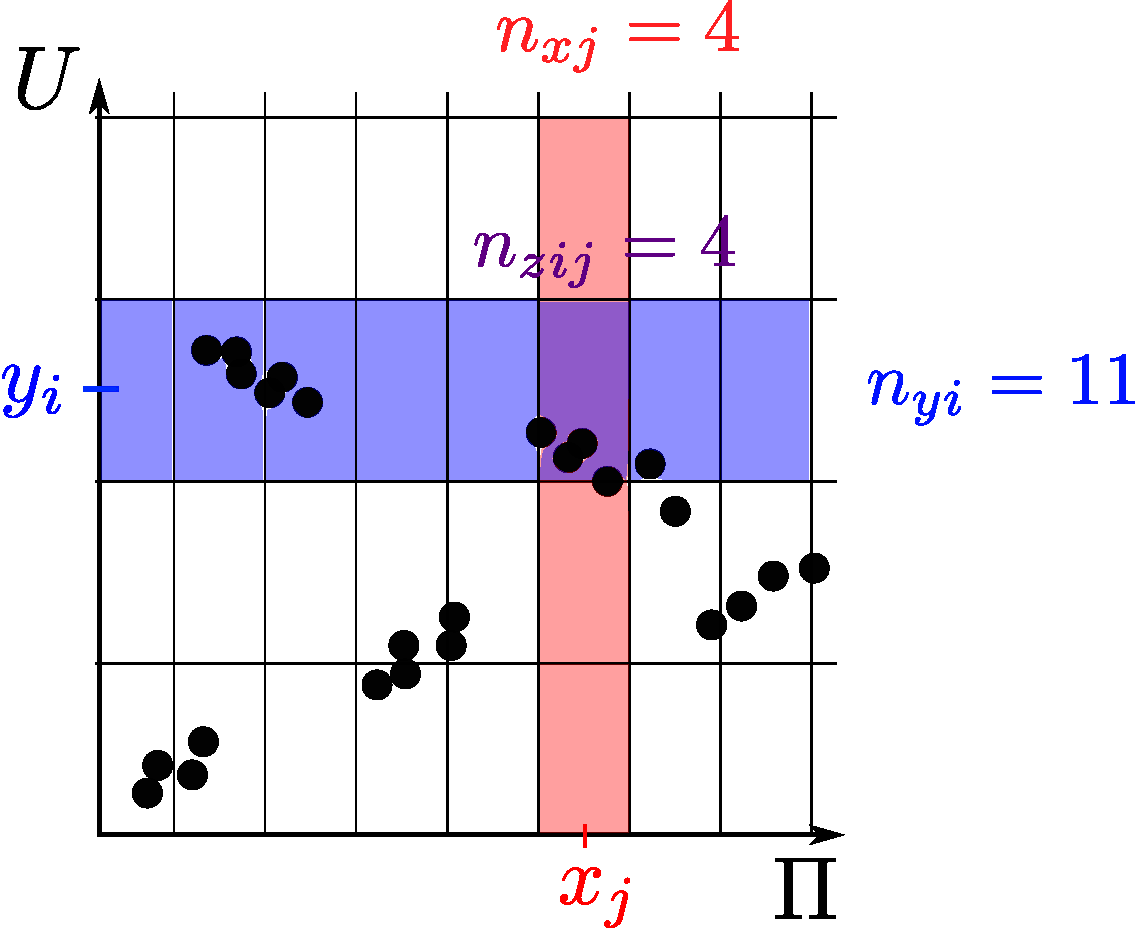
\includegraphics[width=\textwidth]{boxes}
    \caption{Méthode d'estimation par histogrammes des distributions des variables $X$ et $Y$. Les distributions sont estimées à partir de $n_{xj}$, $n_{yi}$ et $n_{zij}$, ce qui permet d'estimer l'information mutuelle et l'entropie de Shannon selon \ref{eq:MI} et \ref{eq:H}}
    \label{fig:binning}  
    \end{minipage}
    \hfill
    \begin{minipage}{0.55\textwidth}    
            \centering
            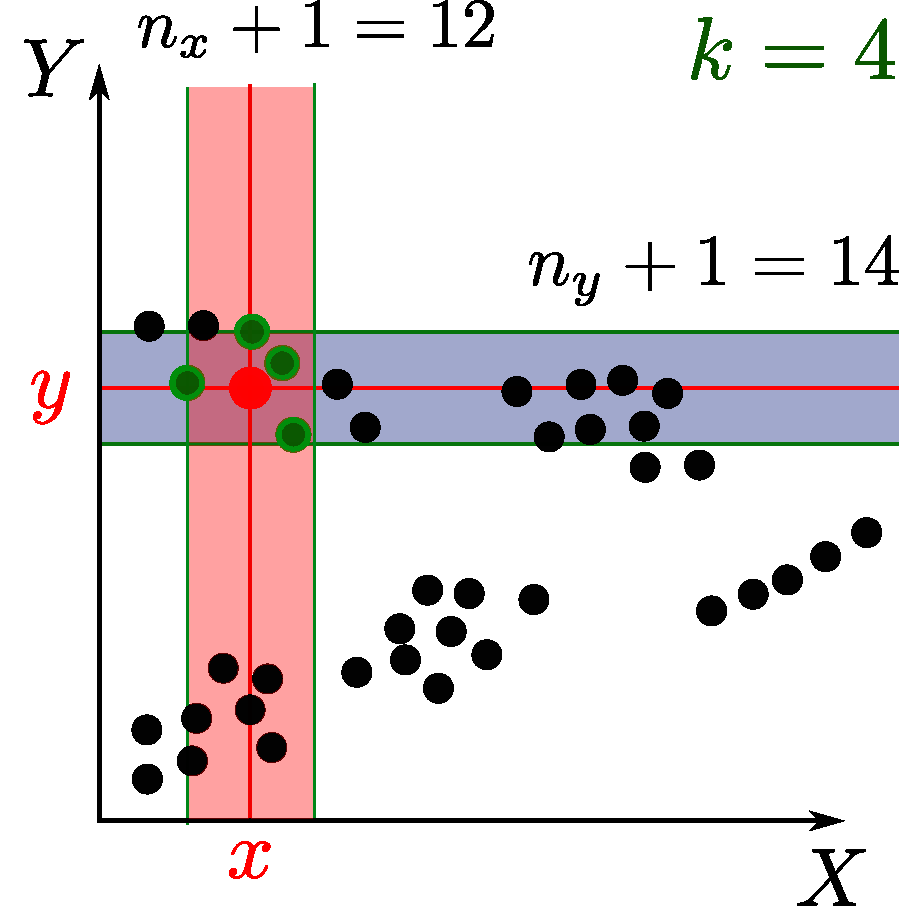
\includegraphics[width=0.55\textwidth]{kraskov.pdf}
            \caption{Méthode d'estimation d'information mutuelle par \emph{k-nearest neighbors}. Les plus proches voisins de chaque point (indiqués en vert pour le point marqué en rouge) déterminent une fenêtre selon chaque axe. Les valeurs de $n_x$ et $n_y$ permettent d'estimer directement l'information mutuelle (voir équation~\ref{eq:knn}).}
            \label{fig:kraskov}
    \end{minipage}
    \end{figure}

L'information mutuelle et l'entropie sont des grandeurs définies à partir de la distribution des variables aléatoires. Nous ne connaissons pas leur distribution et devons donc estimer ces quantités à partir des échantillons de données. 
Nous nous intéresserons en particulier à l'information mutuelle entre les variables $U$ et $\bmu$, qui sont des variables continues. Nous présentons deux méthodes classiques d'estimation de l'information mutuelle pour des variables continues.


Une première méthode d'estimation classique est la méthode des histogrammes (\emph{binning}).
Cette méthode s'appuie sur une estimation de la distribution des variables $X$, $Y$ et la distribution de la variable jointe $(X,Y)$ en discrétisant chacune des variables.
Cette méthode est représentée en figure~\ref{fig:binning}. Les variables $X$ et $Y$ sont discrétisées en \emph{bins} de centres $x_k$ et $y_k$ choisis.
La distribution de chaque variable est alors estimée par~: 
$$P(X = x_i) = \frac{n_{xi}}{N} $$ où $n_{xi}$ est le nombre d'échantillons de $X$ tombant dans le \emph{bin} de centre $x_i$ et $N$ le nombre de points. Le même procédé est réalisé pour $Y$ et $(X,Y)$. La précision de l'estimation peut être améliorée en choisissant des tailles de \emph{bins} variables~; nous utilisons ici la méthode simple avec des \emph{bins} de taille fixe.
Pour des variables à valeurs dans $[0,1]$, les centres sont définis par $x_k = \frac{k}{M}+\frac{1}{2M}$, avec $M$ le nombre de \emph{bins}.
D'après cette discrétisation, l'estimation de l'entropie et l'information mutuelle des variables est calculée selon les équations~\ref{eq:H} et \ref{eq:MI}.
La valeur de cet indicateur est très sensible à la résolution choisie pour le calcul des histogrammes, c'est-à-dire le nombre de \emph{bins}.
Par ailleurs, plus ce nombre de \emph{bins} augmente, plus le nombre de points disponibles pour l'estimation doit augmenter. C'est en particulier le cas lorsque la dimension des entrées augmente~:
le nombre d'échantillons disponibles pour l'estimation doit alors augmenter exponentiellement avec la dimension des variables. En effet, à cause de la faible densité des données, de nombreux \emph{bins} ne contiendront pas de points pour l'estimation alors qu'ils auraient dû en contenir d'après leur distribution théorique, ce qui fausse l'estimation.

Une deuxième méthode plus régulièrement utilisée pour l'estimation de l'information mutuelle est l'estimateur par \emph{K-Nearest Neighbors} \parencite{2004kraskov}.
Cet estimateur ne passe pas par l'estimation de la densité de probabilité, contrairement aux histogrammes, mais estime directement l'information mutuelle.
Le découpage de l'espace se fait en recherchant, pour $N$ valeurs d'échantillons d'un couple $(X,Y)$, les $k$ plus proches voisins. Une information mutuelle locale est calculée dans cette zone de l'espace, suivant une formule permettant d'approximer les différences de logarithme par la fonction digamma $\psi$ : 
$$i_j(X,Y) = \psi(k) - \psi(n_{x_j} + 1) - \psi(n_{y_j} +1) + \psi(N)$$
Cette information mutuelle locale est ensuite moyennée sur l'ensemble des points (en notant $\langle \rangle$ l'opérateur de moyenne) ~: 
\begin{equation}\label{eq:knn}
    \hat{I}(X,Y) = \psi(k) - \langle\psi(n_{x_j} + 1) + \psi(n_{y_j} +1)\rangle + \psi(N)
\end{equation}
    
L'estimateur de Kraskov est moins sensible aux paramètres choisis pour son estimation qui sont le nombre de voisins $k$ considérés \parencite{ross_mutual_2014}.
Enfin, l'information mutuelle étant une grandeur largement utilisée en théorie de l'information, il existe de nombreuses autres méthodes d'estimation possibles~\parencite{Doquire2012ACO}.

\section{\'Evaluation de la relation fonctionnelle entre $U$ et $\bmu$ par le coefficient d'incertitude}

Nous explorons d'abord un indicateur permettant d'évaluer une relation fonctionnelle entre $U$ et $\bmu$, le coefficient d'incertitude \parencite{Theil1961EconomicFA}. 
Cet indicateur est une version normalisée de l'information mutuelle et mesure une relation générale entre deux signaux.

\subsection{Définition du coefficient d'incertitude}

L'information mutuelle $I(U,\bmu)$ mesure une relation quelconque entre les variables $U$ et $\bmu$.
Nous souhaitons normaliser $I(U,\bmu)$ par la valeur maximale qu'elle peut prendre dans une carte, afin d'obtenir un indicateur à valeurs dans $[0,1]$. 
$I(U,\bmu)$ est en effet égale à 0 lorsque les deux variables sont indépendantes et maximale lorsqu'il existe une bijection entre $U$ et $\bmu$.

Si on considère des variables discrètes, cette valeur maximale est $H(U)$, atteinte lorsque $U$ est une fonction de $\bmu$.
En effet, par construction, $\bmu$ est une fonction de $U$ dans une carte de Kohonen~: la recherche de BMU est déterministe. C'est-à-dire, $I(U,\bmu) = I (U, f(U))$.
Par propriété de l'information mutuelle, $I(U,\bmu) \leq I(U,U) = H(U)$
Cette valeur est atteinte si et seulement si $U$ et $\bmu$ sont en bijection, autrement dit, si et seulement si $U$ est aussi une fonction de $\bmu$.

Nous définissons donc l'indicateur $U_c$, marquant la relation fonctionnelle entre $U$ et $\bmu$ comme~:
\begin{equation}
U_c(U|\bmu) = \frac{I(\bmu,U)}{H(U)}
\end{equation}

Ce coefficient n'est pas symétrique et mesure l'information portée par le second terme sur le premier, relativement à la valeur maximale qu'il peut prendre, $H(U)$. 
On a $U_c(U|\bmu) \in [0,1]$. 
Cette variante normalisée de l'information mutuelle correspond en fait au \emph{coefficient d'incertitude} entre $U$ et $\Pi$ et introduit en~\cite{Theil1961EconomicFA}.

$U_c$ vaut 1 lorsque $U$ est une fonction de $\bmu$, et $0$ lorsque les deux distributions sont indépendantes.
Cependant, l'égalité $I(U,U) = H(U)$ est uniquement vraie dans le cas de variables aléatoires discrètes.
Pour l'utilisation de $U_c$ comme indicateur de la relation fonctionnelle, il sera donc nécessaire de considérer $\bmu$ et $U$ comme des variables discrètes et d'estimer l'information mutuelle et l'entropie par la méthode des histogrammes. L'indicateur que nous envisageons sera donc très dépendant des paramètres d'estimation (nombre de \emph{bins}).

\begin{figure}
    \centering
    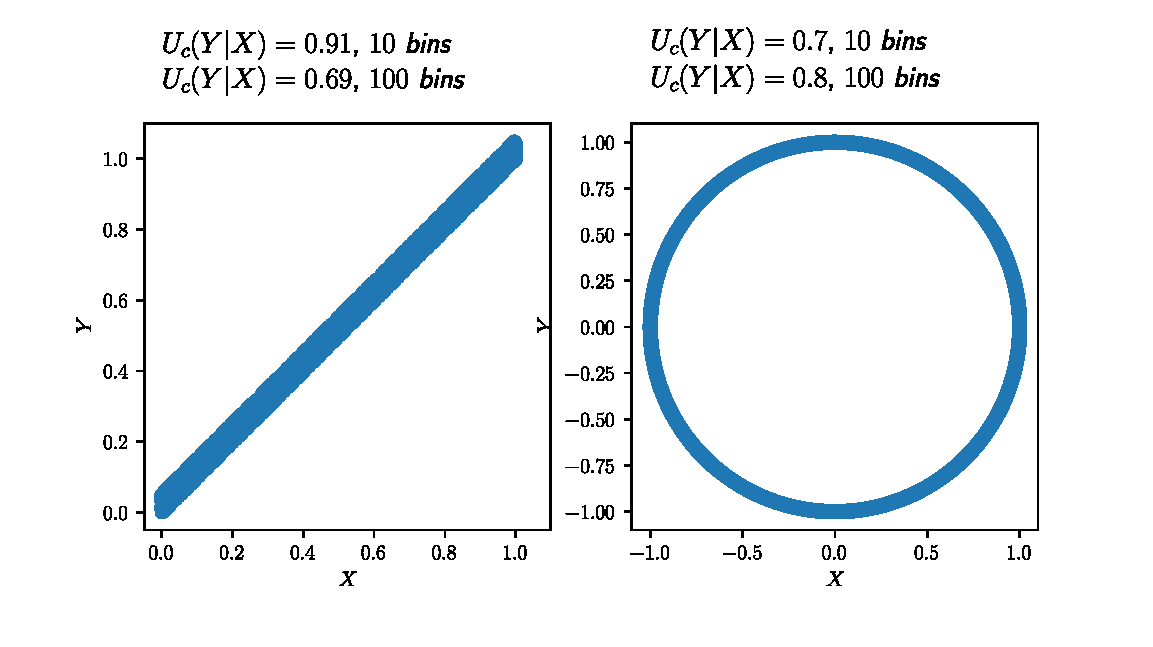
\includegraphics[width=0.75\textwidth]{comparaison_binning.pdf}
    \caption{Comparaison du calcul de $I(X,Y)$ sur deux distributions. \`A gauche, la relation entre $Y$ et $X$ se rapproche d'une fonction, mais bruitée. \`A droite, la relation n'est pas fonctionnelle, mais de telle sorte qu'une valeur de $X$ correspond au maximum à deux valeurs de $Y$.}
    \label{fig:exemple-limite}
    \end{figure}

Afin de choisir ces paramètres d'estimation, décrivons le type de relation fonctionnelle que nous cherchons à mesurer dans une carte de l'architecture.
Nous présentons en figure~\ref{fig:exemple-limite} deux exemples de relations entre des variables aléatoires $X$ et $Y$. Dans le cas de gauche, la relation se rapproche d'une relation fonctionnelle, mais cette relation est bruitée. Une même valeur de $X$ correspond à un intervalle de valeurs de $Y$. Dans le cas de droite, la relation n'est pas une fonction, mais une valeur de $X$ correspond à exactement deux valeurs de $U$. En haut de la figure, nous indiquons le coefficient d'incertitude, calculé pour deux résolutions de discrétisation de $Y$. Dans les deux cas, $X$ est discrétisé en 500 \emph{bins}.
L'indicateur que nous voulons utiliser avec CxSOM doit privilégier la fonction bruitée (à gauche de la figure) par rapport à la relation qui n'est pas fonctionnelle (à droite).
Dans le cas des cartes, nous cherchons en effet à mesurer si une valeur de $\bmu$ correspond à un unique intervalle de $U$, et non plusieurs intervalles comme dans le cas d'une carte simple, dans laquelle deux valeurs de $U$ éloignées sont codées par une même position de BMU, voir figure~\ref{fig:cr_xp}.

Lorsque nous utilisons une discrétisation fine, par exemple de $100$ bins sur la figure, le coefficient d'incertitude calculé dans le cas ou la relation est non-fonctionnelle est inférieur à celui calculé dans le cas de la relation fonctionnelle bruitée~: $U_c(Y|X) = 0.7$.
En effet, une valeur de $X$ correspond à seulement 2 valeurs de\emph{bins} pour $Y$ dans le premier cas, mais un grand nombre de points dans le second cas. La proximité de ces points n'est pas représentée dans le calcul.
Lorsque nous élargissons la taille de discrétisation de $Y$, $U_c(Y|X)$  s'améliore dans le cas de la relation bruitée. Cette discrétisation à gros grain pour $Y$, permet d'ignorer la dispersion locale des valeurs de $Y$.

Pour que $U_c(U|\bmu)$ ne prenne pas en compte un bruit local sur les valeurs de $U$, il faudra donc choisir une discrétisation de $U$ à gros grains. Ces paramètres de discrétisation dépendent de l'organisation des données.
L'indicateur $U_c$ défini ici doit plutôt être considéré comme un indicateur statistique s'inspirant du coefficient d'incertitude que comme une estimation d'une valeur théorique, à cause de ce choix de paramètres et de la discrétisation des variables.

\subsection{Application de  $U_c$ à CxSOM}

\begin{figure}
    \centering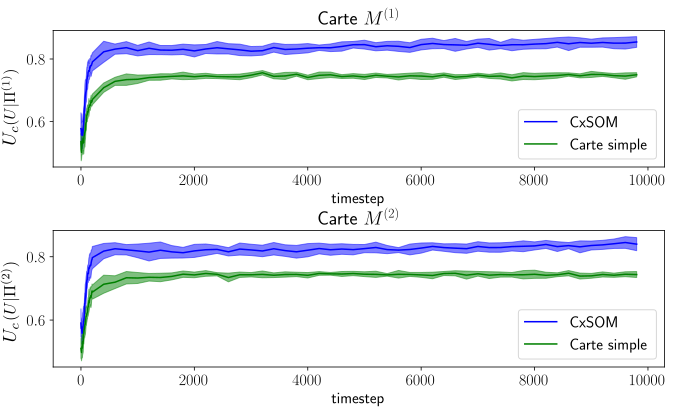
\includegraphics[width=0.8\textwidth]{evolution_MI_2}
    \caption{\'Evolution du coefficient d'incertitude $U_c(U|\bmu)$ dans chaque carte au long de l'apprentissage. L'intervalle de discrétisation choisi pour $U$ est de $0.02$ (50 \emph{bins}).
    La courbe bleue correspond à $U_c(U|\bmu)$ dans l'architecture de cartes $M\m{1}$ et $M\m{2}$, que nous comparons à l'évolution de $U_c$ dans une carte simple apprenant sur les mêmes entrées $\inpx\m{1}$ ou $\inpx\m{2}$.}
    \label{fig:MI_evol}
    \end{figure}

Nous traçons maintenant l'évolution de $U_c(U|\bmu)$ au cours de l'apprentissage dans un système de deux cartes apprenant sur le cercle en deux dimensions, afin de vérifier comment $U_c$ reflète la qualité de l'apprentissage du modèle dans une carte. L'organisation finale de $U$ selon $\bmu$ correspond à celle représentée en figure \ref{fig:cr_xp}.

Pour cela, nous calculons $U_c(U|\bmu\m{1})$ et $U_c(U|\bmu\m{2})$ sur des phases de test réalisées tout au long de l'apprentissage d'une architecture de cartes, comparée à celles calculées sur des cartes simples.
Cette évolution est tracée en figure~\ref{fig:MI_evol}. Ces tracés correspondent à une valeur moyennée sur 10 expériences.
Nous avons discrétisé $U$ en 50 \emph{bins}, et en 500 pour $\bmu\m{i}$~: comme soulevé au paragraphe précédent, il est nécessaire d'utiliser un intervalle plus large pour les valeurs de $U$, afin de ne pas prendre en compte la dispersion des points au niveau local.

Ces tracés montrent que les quantités $U_c(U|\bmu\m{1})$ et $U_c(U|\bmu\m{2})$ sont bien toutes deux plus élevées pour CxSOM, tout au long de l'apprentissage, que dans le cas ou les cartes sont séparées. Les valeurs pour CxSOM s'approchent de 1 à la fin de l'apprentissage, reflétant bien l'observation réalisée que $U$ est une fonction de $\bmu$ dans chaque carte.

\subsection{Discussion}

D'après nos observations, $U_c$ peut certes être utilisé comme indicateur d'une relation fonctionnelle entre $U$ et $\bmu$ dans chaque carte, mais sous réserve de choisir correctement la taille de l'intervalle de discrétisation pour $U$ lors de l'estimation (nombre de \emph{bins})
La taille de cet intervalle de discrétisation doit être assez élevée pour englober le bruit local sur les données, mais suffisamment faible pour détecter une séparation entre deux intervalles de $U$ codés par une même position de BMU.
Le choix de cet intervalle de discrétisation de $U$ a une grande influence sur la valeur de l'indicateur, rendant difficile son utilisation comme valeur quantifiée permettant de comparer des expériences.
Par ailleurs, la discrétisation de $U$ pour des variables de grande dimension nécessiterait un échantillon de grande taille, ce qui limite également son utilisation.
Enfin, l'aspect originellement continu des variables $\bmu$ et $U$ n'est pas pris en compte par cet indicateur, qui nécessite la discrétisation des variables.

Le coefficient d'incertitude n'est donc pas un indicateur adapté à la mesure de la relation fonctionnelle existant entre $U$ et $\bmu$. Bien qu'il s'appuie sur l'information mutuelle, qui mesure une relation quelconque entre des signaux, il ne traduit pas la relation fonctionnelle de la façon dont nous voulons la mesurer dans CxSOM. En particulier, nous voulons prendre en compte l'aspect continu des valeurs de $U$.

Cependant, l'utilisation de l'information mutuelle continue pour évaluer l'apprentissage nous paraît pertinente, mais afin d'évaluer une relation plus générale que la relation fonctionnelle.
Nous explorerons ce calcul en section~\ref{sec:mi}.

\section{\'Evaluation de la relation fonctionnelle entre $U$ et $\bmu$ par le ratio de corrélation}

Au vu des limitations montrées par l'indicateur $U_c$, nous avons choisi de considérer un autre indicateur de la relation fonctionnelle entre $U$ et $\bmu$~: le ratio de corrélation.

\subsection{Définition}

Le ratio de corrélation $\eta(Y;X)$ est un coefficient mesurant une relation fonctionnelle non-linéaire entre deux variables. Il atteint la valeur de 1 lorsque $Y$ est fonction de $X$, et est nul lorsque les deux variables sont statistiquement indépendantes.

La mesure de la dépendance fonctionnelle entre deux variables $X$ et $Y$ peut se décomposer en deux étapes~:
\begin{enumerate}
    \item Trouver une fonction $\varphi(X)$ qui approxime les valeurs de $Y$
    \item Mesurer la qualité de l'approximation.
\end{enumerate}

La fonction approchant le mieux l'ensemble des valeurs $(x,y)$ d'un échantillon de deux variables $(X \in \Omega_X$, $Y \in \Omega_Y)$, au sens des moindres carrés, est la fonction~:
\begin{equation}
    \varphi(x) = \mathbb{E}(Y|X = x), x \in \Omega_X
\end{equation}

Le ratio de corrélation $\eta$ se définit à partir de $\varphi$ et mesure alors la qualité de l'approximation des valeurs de $Y$ par la fonction $\varphi$~:

\begin{equation}\label{eq:cr}
   \eta(Y;X) = \frac{Var(\mathbb{E}(Y|X))}{Var(Y)}
\end{equation}

Une possibilité d'estimation de $\varphi(x)$ est illustré en figure~\ref{fig:cr_box}~: nous discrétiserons les valeurs de $X$ en $n$ valeurs $(x_1, \cdots, x_n)$ et prendrons $\varphi(x_i)$ comme la moyenne des valeurs de $Y$ dans l'intervalle $[x_{i-1}, x_i]$.
Le ratio de corrélation n'est pas symétrique. Par le fait qu'il s'appuie sur un rapport, il n'est pas sensible à une transformation linéaire de $Y$ et est sans unité.

\begin{figure}
    \centering
    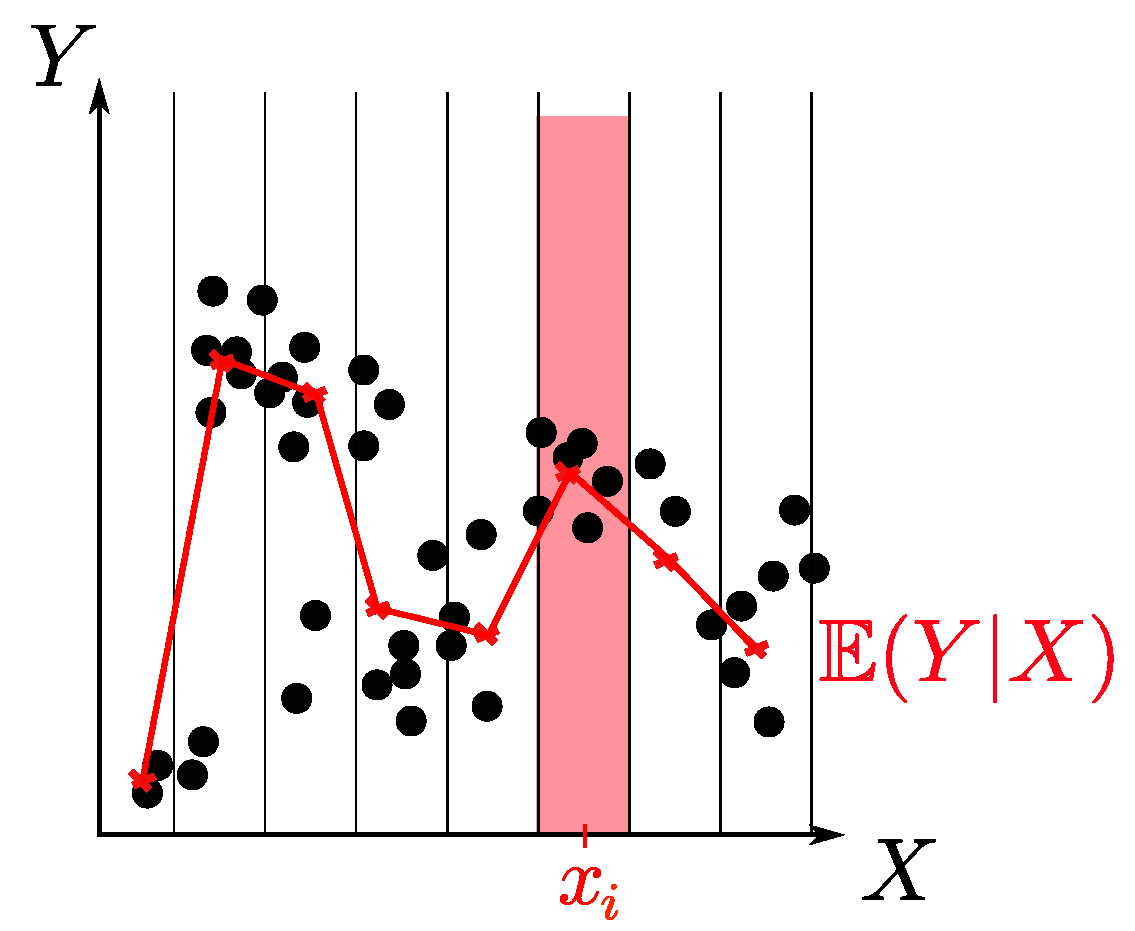
\includegraphics[width=0.5\textwidth]{boxes_CR.pdf}
    \caption{Exemple d'approximation non-linéaire de la relation entre $X$ et $Y$ par $\varphi(x)= \mathbb{E}(Y|X=x)$. Cette approximation est ici réalisée en discrétisant les valeurs de $X$. \label{fig:cr_box}}
\end{figure}

\subsection{Application du ratio de corrélation sur l'architecture de deux cartes}

\begin{figure}
    \centering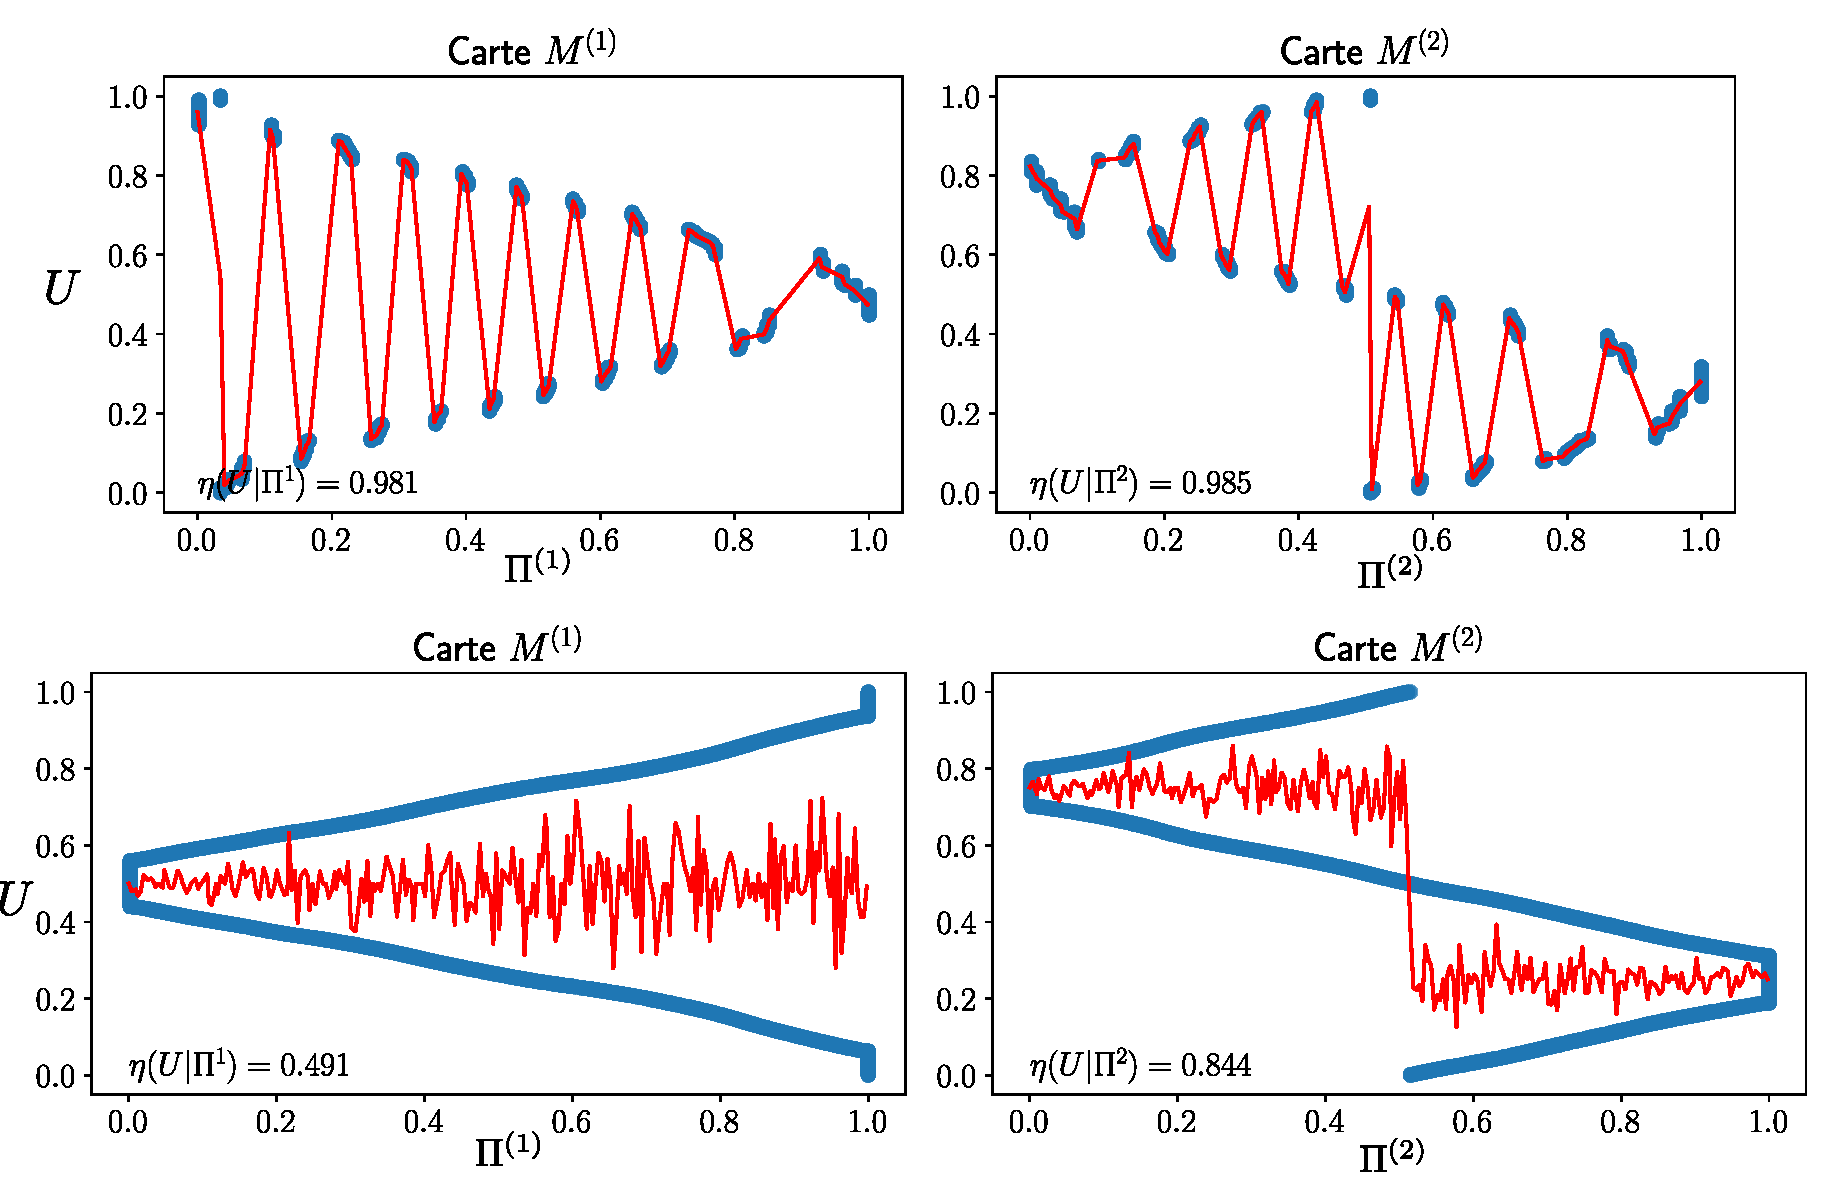
\includegraphics[width=0.8\textwidth]{correlation_ratio_cercle0.pdf}
    \caption{Tracé du ratio de corrélation et de $\varphi$ sur des entrées placées sur un cercle, dans le cas de CxSOM et d'une carte simple. $\varphi(p) = \mathbb{E}(U|\bmu =p)$ est tracée en rouge.
    Nous observons que $\varphi(p)$ permet bien d'approximer la relation fonctionnelle existant dans CxSOM, en haut, ce qui se traduit sur la valeur du ratio de corrélation~: $\eta(U;\bmu\m{1}) = 0.98$, $\eta(U;\bmu\m{2}) = 0.99$. Au contraire, le ratio de corrélation est plus faible dans le cas des cartes simples, en bas.
     \label{fig:cr_xp}}
\end{figure}

\begin{figure}
   \centering 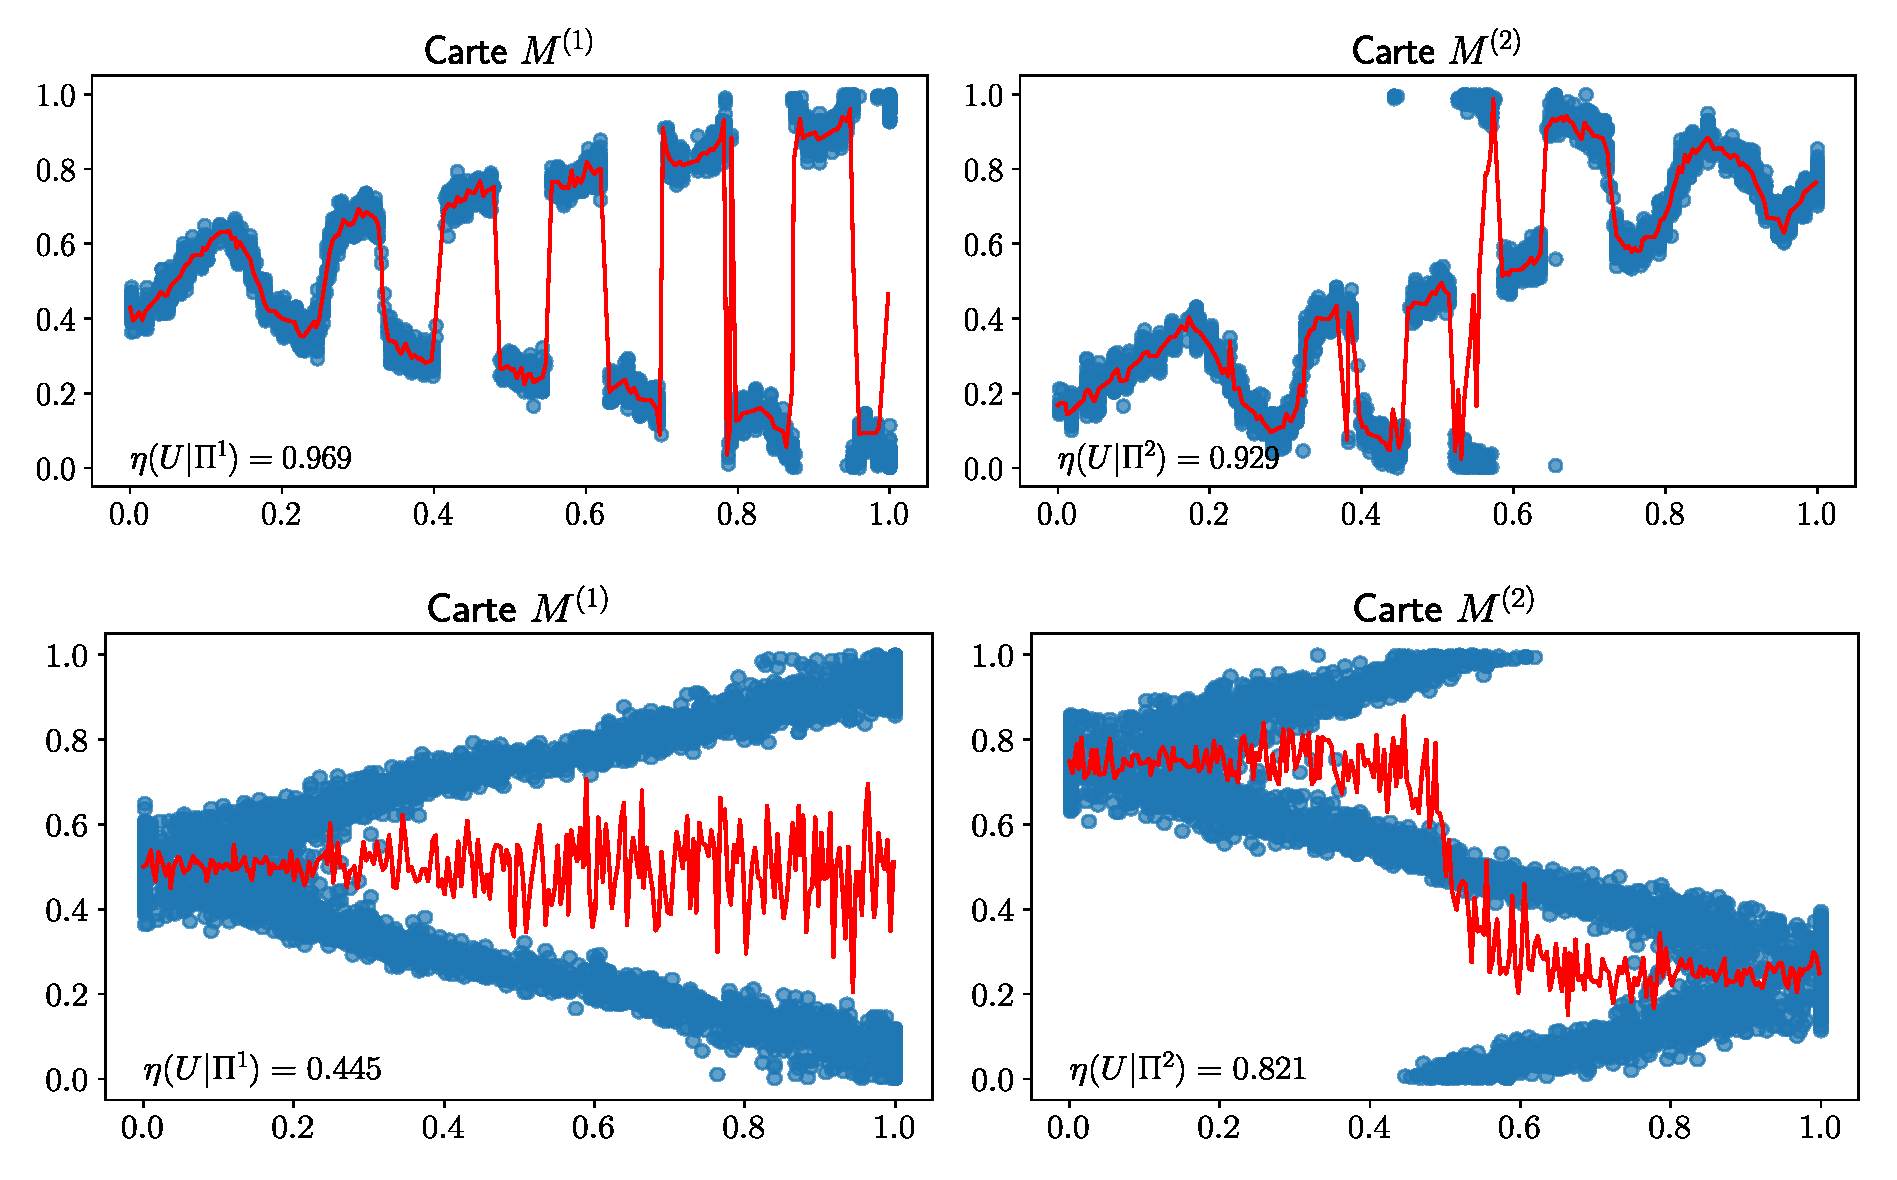
\includegraphics[width=0.8\textwidth]{xu_yu_both_anneau.pdf}
    \caption{Tracé du ratio de corrélation et de $\varphi$ sur des entrées placées sur un anneau, dans le cas de CxSOM et d'une carte simple. Les données d'entrées sont bruitées, ce qui conduit à une dispersion plus élevée de $U$ pour chaque valeur de $\bmu$, tout en restant dans un seul intervalle. Le ratio de corrélation traduit toujours correctement que la relation entre $U$ et $\bmu$ s'approche d'une fonction et reste plus élevé que dans le cas des cartes simples. \label{fig:cr_bruit}}
\end{figure}

Nous utilisons à présent le ratio de corrélation pour quantifier la relation fonctionnelle entre $U$ et $\bmu\m{i}$, sur une architecture de deux cartes après apprentissage. Le but ici est d'illustrer comment cet indicateur traduit les observations réalisées graphiquement, afin de valider son utilisation et de comprendre ce qu'il représente.

Nous reprenons trois exemples de modèles d'entrées tirés du chapitre précédent~:
\begin{itemize}
    \item Lorsque les entrées sont tirées sur le cercle de centre 0.5 et de rayon 0.5 (Entrées \textbf{A}, figure~\ref{fig:inputs}). $U$ correspond à l'angle du point sur le cercle.
    \item Lorsque les entrées sont tirées sur un anneau, construit en ajoutant un bruit aux points de centre 0.5 et de rayon 0.5. (Entrées \textbf{F}) $U$ correspond également à l'angle du point sur le cercle et l'indicateur doit pouvoir refléter l'apprentissage de $U$ malgré le bruit sur les entrées.
    \item Lorsque les entrées sont tirées sur une courbe de Lissajous (Entrées \textbf{D}).
\end{itemize}

Nous comparerons les valeurs du ratio de corrélation obtenues dans l'architecture, à celui obtenu dans le cas de deux cartes simples qui prennent $\inpx\m{1}$ ou $\inpx\m{2}$ en entrées. 
Nous rappelons que dans ce dernier cas, les cartes ne font pas apparaître de relation fonctionnelle entre $U$ et $\bmu$.

Nous représentons d'abord le tracé de $U$ selon $\bmu$ dans chaque carte, après apprentissage, en figure~\ref{fig:cr_xp} pour le cercle et en figure \ref{fig:cr_bruit} pour l'anneau. (Voir figure~\ref{fig:u_bmu_lissa} pour la courbe de Lissajous).
Nous y traçons également la fonction $\mathbb{E}(U|\bmu)$, qui approxime le nuage de points par une fonction. 
Les valeurs des ratios de corrélation calculés dans chacun des cas sont indiqués au tableau~\ref{tab:eta}.
Nous y ajoutons également les valeurs de $\eta(U;\inpx\m{1})$ et $\eta(U;\inpx\m{2})$, qui quantifient la relation initiale entre chaque entrée et $U$.


Nous observons sur ces tracés que la relation fonctionnelle entre $U$ et $\bmu$ est bien approximée par $\mathbb{E}(U|\bmu)$ dans le cas de l'architecture de cartes. Les valeurs de $\eta(U;\bmu\m{1})$ et $\eta(U;\bmu\m{2})$ sont alors proches de 1. 
Dans le cas de l'anneau, $\mathbb{E}(U|\bmu)$ approxime également bien la relation entre les entrées, ce qui se traduit sur la valeur de l'indicateur~: $\eta(U;\bmu\m{1}) = 0.96$ et  $\eta(U;\bmu\m{1}) = 0.94$. 
L'indicateur différencie donc bien le bruit local sur $U$, de l'existence de deux valeurs séparées de $U$ pour une même position $\bmu$.

Dans le tableau, nous notons par contre que $\eta(U;\inpx\m{2}) \approx 0.8$ dans chacun des modèles d'entrées~; cette valeur est proche de $1$, alors que la relation n'est pas \og plus fonctionnelle \fg{} que celle existant entre $U$ et $\inpx\m{1}$, pour laquelle $\eta(U;\inpx\m{1}) \approx 0.4$. Intuitivement, on s'attendrait à ce qu'un indicateur prenne une valeur similaire pour $\eta(U;\inpx\m{1})$ et $\eta(U;\inpx\m{2})$. Cette observation suggère que la valeur seule du ratio de corrélation nous permet mal de quantifier de valeur absolue la qualité de la relation fonctionnelle.
Le ratio de corrélation apparaît donc comme un bon indicateur de la relation fonctionnelle entre $U$ et $\bmu\m{i}$, mais sa valeur devra être comparée à $\eta(U;\inpx\m{i})$ pour pouvoir l'interpréter.

\begin{table}
    \centering
    \caption{Comparaison des valeurs du ratio de corrélation sur plusieurs expériences.\label{tab:eta}}
    \begin{tabular}{*7c}
        \toprule
        & \multicolumn{2}{c}{Entrées} & \multicolumn{2}{c}{CxSOM} & \multicolumn{2}{c}{Cartes Simples} \\
        \cmidrule(lr){2-7}
         & $\eta(U;\inpx\m{1})$ & $\eta(U;\inpx\m{2})$  & $\eta(U;\bmu\m{1})$ & $\eta(U;\bmu\m{2})$  & $\eta(U;\bmu\m{1})$ & $\eta(U;\bmu\m{2})$ \\    
        \midrule
        Cercle &   $0.45 $    & $0.84$  &  $0.98$ & $0.99$ & $0.49$ & $0.84$      \\
        Anneau &  $0.43$      &  $0.83$      & $0.97$ & $0.93$ & $0.44$ & $0.82$ \\
        Lissajous &  $0.81$     &  $0.80$ & $0.96$ & $0.94$  & & \\
        \bottomrule
    \end{tabular}
\end{table}

Enfin, nous traçons en figure~\ref{fig:cr_evol} l'évolution du ratio de corrélation sur les 200 premiers pas d'apprentissage des cartes. 
Nous observons que $\eta(U;\bmu)$ garde une valeur élevée tout au long de l'apprentissage pour CxSOM.
Le ratio de corrélation ne traduit donc pas l'organisation des poids.
En effet, il ne prend pas en compte la proximité des positions. Deux valeurs discrétisées de $\bmu$ ont la même influence dans le calcul, qu'elles soient proches ou distantes dans la carte.
Or, chaque carte définit son BMU en fonction de $\inpx\m{1}$ et de son entrée contextuelle $\bmu\m{2}$, qui représente directement $\inpx\m{2}$, même au début de l'apprentissage. $U$ est donc une fonction du BMU dans chaque carte dès le début de l'apprentissage, ce qui est observé sur la courbe d'évolution.

\begin{figure}
    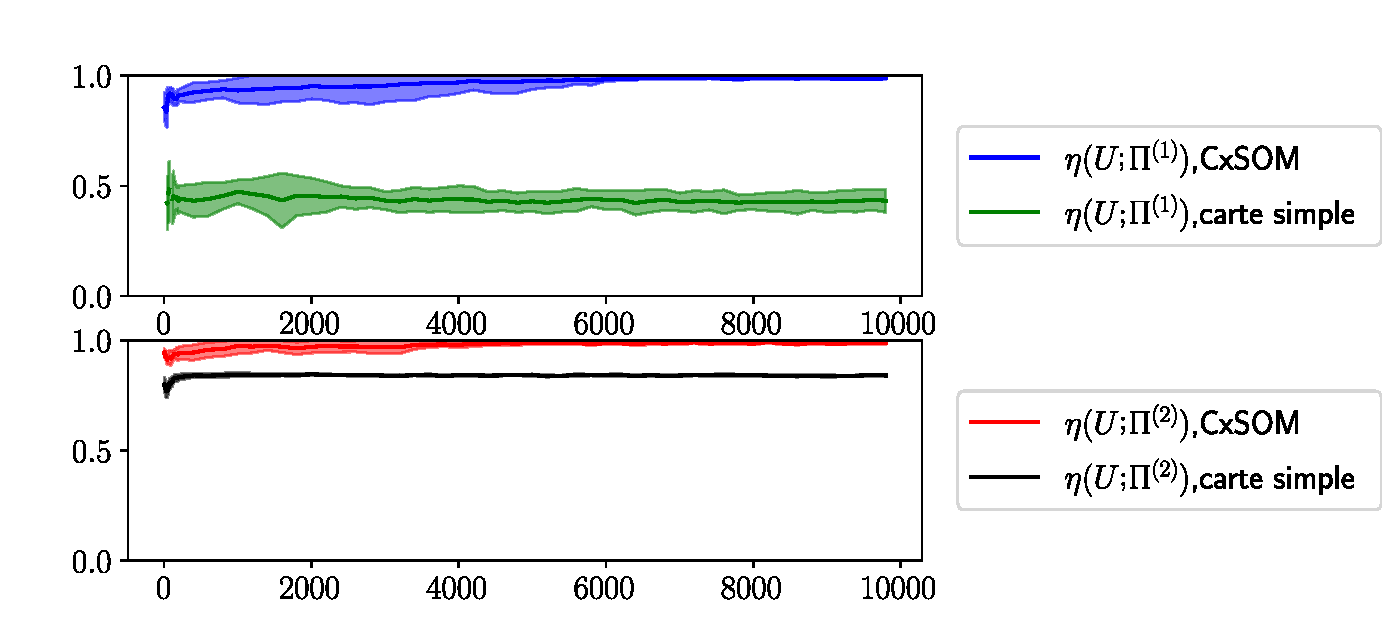
\includegraphics[width=\textwidth]{cr_evol.pdf}
    \caption{\'Evolution du ratio de corrélation pendant l'apprentissage d'une architecture de deux cartes sur des entrées en cercle. Les tracés correspondent à la moyenne et l'écart-type du ratio, calculés sur 10 expériences. Le ratio de corrélation reste plus faible dans les cartes simples que dans les cartes CxSOM. Il garde une valeur élevée tout au long de l'apprentissage~: le ratio de corrélation ne traduit pas l'organisation des poids, mais vérifie simplement si une carte a un BMU différent pour chaque valeur de $U$. \label{fig:cr_evol}}
\end{figure}

\subsection{Discussion}

Le ratio de corrélation $\eta(U;\bmu)$ est une mesure statistique qui exprime par définition la relation fonctionnelle existant entre $U$ et $\bmu$, ce que nous cherchions à mesurer. 
Cette mesure nécessite de discrétiser les valeurs de $\Pi$, mais pas celles de $U$ 
L'aspect continu de $U$ est donc bien traduit par $\eta$, contrairement à $U_c$.
Il est adaptable pour des cartes en 2D, ainsi que des $U$ en grande dimension.
Il s'agit donc d'une mesure appropriée de la relation fonctionnelle entre $U$ et $\bmu$ dans chaque carte.
Cependant, l'utilisation du ratio de corrélation comme indicateur d'un apprentissage de $U$ par $\bmu\m{i}$ n'est pertinent qu'en le comparant qu'à une valeur d'entrée $\eta(U;\inpx\m{i})$, ou à la valeur qu'il prend dans une carte auto-organisatrice indépendante. 
Par ailleurs, il traduit le caractère continu de $U$ mais pas de $\bmu$. Il ne traduit donc pas l'organisation des poids lors de l'apprentissage. 
Nous pourrions par exemple calculer ce coefficient sur une fenêtre glissante sur $\bmu$ afin de mieux représenter cette continuité.

En conclusion, nous cherchions un indicateur numérique permettant de quantifier l'encodage du modèle d'entrée dans chaque carte, afin de caractériser des expériences pour lesquelles $U$ est de grande dimension, et d'avoir une valeur numérique permettant de comparer plusieurs expériences et d'optimiser les paramètres de l'architecture.
Le ratio de corrélation est ainsi un indicateur beaucoup plus adapté que le coefficient d'incertitude pour la mesure de la relation fonctionnelle entre $U$ et $\bmu$ dans chaque carte. Cette relation fonctionnelle est caractéristique de l'apprentissage de la relation entre les entrées dans des architectures de deux et trois cartes.
Cependant, il faut noter que sa valeur n'est pas absolue et doit être comparée à la valeur qu'il prend initialement dans le modèle d'entrées.

\section{Comment utiliser l'information mutuelle continue comme indicateur d'un apprentissage ?}

Le ratio de corrélation et le coefficient d'incertitude ont proposé deux manières différentes de mesurer le fait que $U$ est une fonction du BMU dans chaque carte.
Bien que le coefficient d'incertitude $U_c$ s'appuie sur l'information mutuelle, l'indicateur que nous avons présenté n'en est pas une véritable estimation, par la discrétisation à gros grains de $U$.

Sur des architectures à plus de trois cartes, il n'est pas certain ni même souhaitable que $U$ soit une fonction de la position du BMU dans toutes les cartes d'une architecture, mais plutôt que la représentation de $U$ soit distribuée entre les cartes, tout en présentant de la redondance en terme d'information.
Nous envisageons donc dans cette section des perspectives d'utilisation de l'information mutuelle entre $U$ et les positions des BMUs $(\bmu\m{1}, \bmu\m{2})$ pour analyser l'apprentissage du modèle dans une architecture de cartes.

\subsection{\'Evolution de l'information mutuelle entre $U$ et $\bmu$ au cours d'un apprentissage}

\begin{figure}
    \centering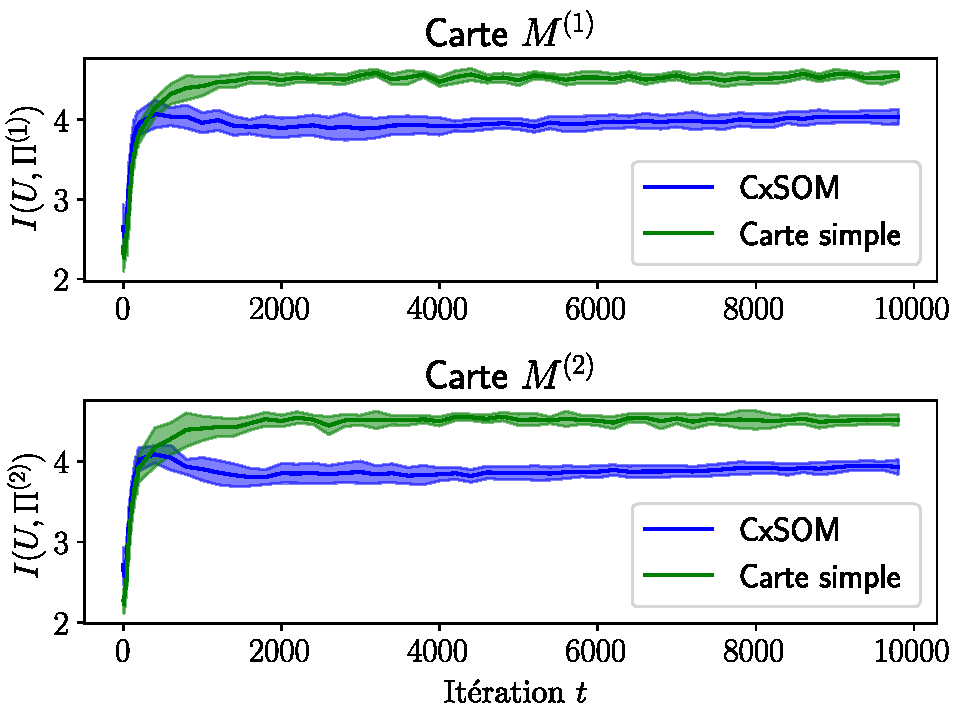
\includegraphics[width=0.8\textwidth]{evolution_MI_K_2}
    \caption{\'Evolution de $I(U,\bmu)$ dans chaque carte au long de l'apprentissage, estimé par la méthode des KNN (cf.~\ref{eq:knn}).
    Sa valeur est moyennée sur 10 expériences. Nous comparons les valeurs obtenues dans une architecture CxSOM, en bleu, au cas d'une carte apprenant indépendamment sur les mêmes entrées $\inpx\m{1}$ ou $\inpx\m{2}$.
    Le même échantillon $U$ a été utilisé lors de chaque phase de test pour une même expérience.
    Nous observons que les positions des BMUs d'une carte indépendante partagent plus d'information avec $U$ que dans le cas de CxSOM.
    \label{fig:MI_evol_total}}
    \end{figure}

Nous nous intéressons à l'information mutuelle continue entre $U$ et $\bmu$, que nous estimons grâce à la méthode des KNN, présentée en section~\ref{sec:estimation}. Contrairement à l'estimation à gros grains réalisée en section précédente pour $U_c$, il s'agit maintenant d'une véritable estimation de la valeur de l'information mutuelle entre les deux variables continues que sont $\bmu$ et $U$.

En figure~\ref{fig:MI_evol_total}, nous traçons l'évolution de l'information mutuelle dans les deux cartes au cours de phases de test réalisées tout au long de l'apprentissage.
Nous observons que l'information mutuelle entre $U$ et $\bmu$ évolue vers une valeur qui est plus élevée dans une carte isolée que dans une architecture CxSOM.
Ce résultat est étonnant~: cela signifie donc que chaque carte au sein de CxSOM encode en fait moins d'information sur le modèle d'entrées qu'une carte isolée, qui ne reçoit pourtant que l'entrée $\inpx\m{1}$ ou $\inpx\m{2}$, c'est-à-dire une partie du modèle.
Nous interprétons ce résultat par le fait que l'information apprise sur le modèle par une carte n'est pas répartie de la même façon dans les deux expériences.
Dans une carte indépendante, le niveau de quantification vectorielle sur $\inpx$ est plus précis que celui que nous avions observé dans CxSOM.
Or, l'encodage de la valeur $\inpx$ donne déjà beaucoup d'information sur le modèle $U$.
Dans CxSOM, on perd ce niveau de quantification sur $\inpx$, ce qu'on a observé en figure~\ref{fig:erreur}. On perd donc de l'information sur $\inpx$.

Le fait que l'information mutuelle soit plus élevée dans une carte indépendante dans les deux expériences traduirait ainsi une perte d'information sur l'entrée $\inpx$ dans CxSOM par rapport à une carte simple, à cause de la perte de précision en quantification vectorielle. 
La valeur de l'information mutuelle comprend à la fois le gain d'information qui existe sur $\inpx\m{2}$ au sein de $M\m{1}$, donc sur $U$ (et inversement), et la perte d'information sur $\inpx\m{1}$. 
Il est probable que cette perte d'information domine dans le calcul, d'où la perte globale d'information.
Les cartes effectueraient donc un compromis~: chacune gagne de l'information sur le modèle $U$, au détriment de l'information apprise sur l'entrée externe.

Afin de mieux analyser l'apprentissage du modèle d'entrées par les cartes, nous pouvons envisager des méthodes permettant de séparer l'information entre variables. Elles nous permettraient de mesurer le gain d'information sur $U$ dans une ou plusieurs cartes sans s'intéresser à l'information gagnée ou perdue sur l'entrée externe $\inpx$.
Nous avions en fait utilisé une méthode de séparation de cette information lors de l'estimation du coefficient d'incertitude $U_c$~: le fait de discrétiser grossièrement la distribution de $U$ a permis de mesurer le gain d'information sur $U$, sans prendre en compte l'affaiblissement de la précision de la quantification de l'entrée externe.

Cette perte d'information pose néanmoins une question concernant la création d'architectures contenant de nombreuses cartes et $U$ de grande dimension~: jusqu'à quel point une carte peut-elle se permettre de perdre de l'information sur l'entrée externe pour gagner de l'information sur le modèle ? 
Cette observation renforce l'idée que l'encodage d'une variable $U$ en grande dimension dans une architecture devra être distribué entre les cartes et ne peut être réalisé indépendamment dans chaque carte. D'après les seules observations réalisées sur deux et trois cartes dans cette thèse, nous ne pouvons pas affirmer ou non si cette propriété sera vérifiée, en raison de la taille de l'architecture.
Cela constitue une perspective de travaux futurs pour le développement du modèle.

\subsection{Ouvertures possibles}

\begin{figure}
    \centering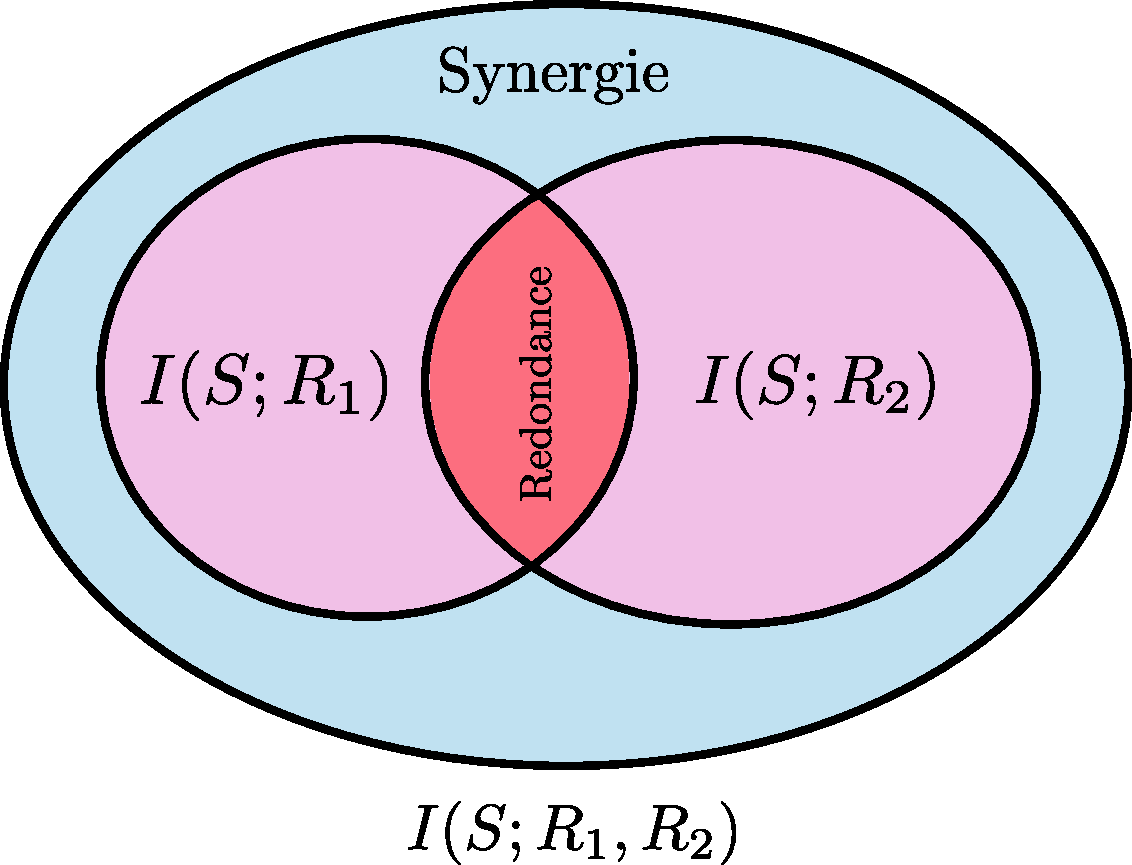
\includegraphics[width=0.5\textwidth]{redondance}
    \caption{Illustration des notions d'information \emph{redondante} et \emph{synergique} entre une variable $S$ et deux variables $R_1$ et $R_2$, schéma adapté de \cite{williams_nonnegative_2010}. Ces travaux définissent une façon de séparer l'information que portent des variables $R_1$ et $R_2$ sur une source $S$. La redondance est l'information apportée à la fois par $R_1$ et $R_2$; la synergie est celle qui n'est apportée que par leur jointure $(R_1,R_2)$. \label{fig:redondance}
    }
\end{figure}

Les mesures proposées dans ce chapitre ont permis d'évaluer un apprentissage du modèle indépendamment dans chaque carte. La mesure de l'information mutuelle dans une architecture de cartes ne se réduit pas au calcul de $I(U,\bmu)$~; de nombreuses grandeurs nous semblent intéressantes à explorer pour une meilleure compréhension de l'apprentissage du modèle dans des architectures comportant plus de cartes.

Nous pouvons tout d'abord noter que la méthode d'estimation par KNN présentée dans ce chapitre est une méthode classique d'estimation de l'information, mais il existe de nombreuses autres méthodes \parencite{Doquire2012ACO}. Des méthodes ont également été développées pour la mesure de l'information mutuelle entre variables continues et discrètes \parencite{ross_mutual_2014, Gao2017EstimatingMI}. Enfin, l'information mutuelle a été utilisée pour analyser l'apprentissage de réseaux de neurones profonds en \cite{ShwartzZiv2017OpeningTB} ou encore directement comme métrique d'apprentissage en \cite{Hjelm2018LearningDR}.
Cette grandeur est ainsi bien documentée et donc pertinente à utiliser dans des travaux futurs.

Ensuite, nous avons soulevé le besoin de séparer les sources d'information sur $U$ et d'étudier son encodage distribué dans l'architecture. Il serait possible de s'intéresser à la notion d'information mutuelle multivariée~: étant donné une variable cible $S$ et deux variables $R_1$ et $R_2$, $I(S;R_1,R_2)$ désigne l'information mutuelle entre $S$ et la variable jointe $(R_1,R_2)$. 
Nous pourrons par exemple mesurer $I(U; \bmu\m{1}, \bmu\m{2})$.
Il est également possible de décomposer cette information multivariée~: \cite{williams_nonnegative_2010} définit, en plus de l'information mutuelle, la notion de redondance et de synergie entre variables, illustrée en figure \ref{fig:redondance}.
La redondance est l'information sur $S$ portée à la fois par $R_1$ et par $R_2$, et la synergie l'information portée seulement par la jointure des variables $R_1$ et $R_2$. Le calcul de telles grandeurs permettrait de séparer l'information gagnée sur $U$ et $\inpx$ dans une carte.
Le calcul de ces grandeurs entre les entrées, le modèle d'entrée et les BMUs des cartes CxSOM sont donc une piste d'étude pour une compréhension de l'encodage de l'information dans une architecture de cartes et pour la définition d'un indicateur ciblant spécifiquement le gain d'information sur $U$ lors de l'apprentissage.


\section{Conclusion}

Ce chapitre utilise la méthode de représentation des éléments des cartes comme des variables aléatoires proposée au chapitre \ref{chap:repr} pour proposer des indicateurs de l'apprentissage multimodal au sein de l'architecture.
Les représentations visuelles sont en effet limitées dans des architectures de plus de deux ou trois cartes, et pour des données en plus grande dimension. La définition d'un indicateur permettra également de comparer l'apprentissage d'architecture, autorisant par exemple l'optimisation automatique des paramètres de l'architecture de cartes.

Dans ce chapitre, nous avons introduit deux indicateurs permettant de mesurer que $U$ est une fonction du $\bmu$ dans chacune des cartes de l'architecture~: le ratio de corrélation $\eta(U;\bmu)$ et le coefficient d'incertitude $U_c(U|\bmu)$.
Nous avons en effet observé dans les deux chapitres précédents que ce comportement marque l'apprentissage du modèle dans des architectures de deux ou trois cartes en une dimension.
Le coefficient d'incertitude est une version normalisée de l'information mutuelle. Il doit être estimé par histogrammes et est donc très sensible aux paramètres d'estimation, ce qui rend son utilisation peu adaptée comme indicateur. De plus, la discrétisation de $U$ est difficilement réalisable pour des variables de grande dimension.
Le ratio de corrélation permet de mesurer directement la relation fonctionnelle entre $U$ et $\bmu$, en passant par l'estimation de $\mathbb{E}(U|\bmu)$.
Dans un but de mesure de la relation fonctionnelle entre $U$ et $\bmu$, nous avons observé que le ratio de corrélation est à privilégier, car il est estimable pour des valeurs de $U$ en toute dimension et ne dépend pas de la taille d'intervalle choisie pour $U$. Sa valeur devra cependant être comparée aux valeurs du ratio de corrélation sur les données d'entrée $\eta(U;\inpx)$.

La relation fonctionnelle entre $U$ et $\bmu$ n'est toutefois pas une propriété souhaitable dans des plus grandes architectures ou des $U$ de plus grande dimension, car elle semble induire une forte perte d'information sur l'entrée externe au profit d'un grain d'information sur le modèle. 
On voudrait plutôt que la représentation de $U$ soit distribuée entre les cartes.
Pour étudier l'apprentissage multimodal dans un cadre plus général, nous suggérons aux travaux futurs de s'intéresser à des mesures d'information mutuelle multivariée entre $U$ et toutes les valeurs des BMUs $(\bmu\m{1}, \cdots, \bmu\m{n})$ au sein des architectures de cartes.

Finalement, ce chapitre montre que la représentation des éléments d'une carte et des entrées d'un point de vue statistique que nous avons proposé au chapitre \ref{chap:repr} est une méthode pertinente pour la compréhension des comportements d'apprentissage du modèle CxSOM.
Cette approche \og comportementale \fg{}, et non basée sur les poids des cartes, rapproche l'étude des cartes de Kohonen et de CxSOM des algorithmes d'apprentissage supervisés, dont les entrées et sorties sont définies.
Les perspectives d'études par l'information mutuelle mentionnées ci-dessus sont donc générales à tout type d'architecture d'apprentissage. 

\ifSubfilesClassLoaded{
    \printbibliography
    %\externaldocument{../main.tex}   
}{}
\end{document}


% Nous avons observé que l'apprentissage du modèle dans deux et trois cartes se caractérise par le fait que chaque carte dissocie les BMUs en fonction du modèle d'entrée $U$ et non seulement de son entrée externe. 
% La variable cachée $U$, représentant le modèle d'entrées, est alors une fonction du BMU $\bmu$ dans chacune des cartes de l'architecture, comme rappelé sur la figure~\ref{fig:upi_chap4}.
% Nous souhaitons définir un indicateur numérique caractérisant cette propriété, c'est-à-dire caractérisant que $U$ est fonction de $\bmu$ dans chaque carte. 

% Nous avons défini les expériences en termes de variables aléatoires. La théorie de l'information de Shannon \cite{Shannon1948AMT} apporte un modèle mathématique qui permet de manipuler et encoder ces variables et quantifier l'information partagée entre leurs distributions.
% Nous proposerons dans ce chapitre des indicateurs permettant d'évaluer l'apprentissage du modèle par l'architecture de cartes. 
% $\mathbb{E}(Var(Y|X))$ représente la moyenne des écarts de $Y|X=x_i$ à sa valeur moyenne en $x_i$ $\mathbb{E}(Y|X=x_i)$ pour une valeur de $X = x_i$ donnée. 
% En effet, en notant $Z$ la variable aléatoire $Y | X=x_i$~: 
% $$ Var(Y|X=x_i) = \mathbb{E}((Z - \mathbb{E}(Z))^2)$$
% $$ Var(Y|X=x_i) = \mathbb{E}((Z - \varphi(x_i))^2)$$

% Lorsque la dépendance entre $Y$ et $X$ est fonctionnelle, les valeurs de $Y|X = x_i$ sont très proches de $\varphi(x_i)$  pour toutes les valeur de $x_i$ et $\mathbb{E}(Var(Y|X=x_i))$ est faible partout. La variance est nulle lorsqu'une valeur de $X$ correspond à un seul point pour $Y$, c'est-à-dire une relation fonctionnelle. 
% Inversement, quand $Y$ et $X$ sont indépendantes, $Var(Y|X=x_i) = Var(Y)$ pour tout $x_i$, donc $\mathbb{E}(Var(Y|X)) = Var(Y)$ et $\eta(Y;X) = 0$.

% La définition du coefficient se retrouve plus généralement sous une forme modifiée de l'équation~\ref{eq:cr}~:
% par la définition des variances conditionnelles,
% $$Var(Y) = \mathbb{E}(Var(Y|X)) + Var(\mathbb{E}(Y|X))$$
% Soit~:
% \begin{equation}
%     \eta(Y;X) = \frac{Var(\mathbb{E}(Y|X))}{Var(Y)}
% \end{equation}